\section{Theorie}
\label{sec:Theorie}
Ziel des vorliegenden Versuches ist die Analyse des gedämpften Schwingkreises.
Dafür soll die Dämpfung, der aperiodische Grenzfall und die Frequenzabhängigkeit des RCL-Kreises untersucht werden.\\
\\
Der grundlegende Aufbau eines Schwingkreises enthält eine Kapazität $C$ und eine Induktivität $L$, wie in Abbildung \ref{fig:unged} zu sehen.
\begin{figure}
    \centering
    \caption{Aufbau ungedämpfer Schwingkreis \cite{}} 
    \label{fig:unged}
    \includegraphics[width = 0.5\textwidth]{pics/aufbau ungedämfter schwingkreis.png}
\end{figure}
Da beide Komponenten Energiespeicher sind, kann durch hineinpumpen eines Energiebetrages eine Schwingung der Energie vollführt werden.
Wird dem System ein Widerstand hinzugefügt, kommt es zu einer gedämpften Schwingung. Das lösen der Differentialgleichung
\begin{equation}
    L \frac{\symup{d}^2 I}{\symup{d} t^2} + \frac{R}{L} \frac{\symup{d} I}{\symup{d} t} + \frac{I}{LC}=0
\end{equation}
für den Strom des Systems, liefert für $I(t)$
\begin{equation}
    I(t)=e^{-t \frac{R}{2L}} \left(I_1 e^{i t \sqrt{\frac{1}{L C} - \frac{R^2}{4 L^2}}}+ I_2 e^{-i t \sqrt{\frac{1}{L C} - \frac{R^2}{4 L^2}}} \right) \, .
\end{equation}
Es wird ersichtlich, dass drei Fälle vorliegen. Ist $ \sfrac{1}{LC}> \sfrac{R^2}{4 L^2}$ ergibt sich der Schwingfall
\begin{equation}
    I(t)=A_0 e^{- 2 \pi \mu t} \cdot \cos(2 \pi \nu t + \eta) \, 
\end{equation}
dabei ist $\eta$ eine Phasenverschiebung, $\mu=\sfrac{R}{4 \pi L}$ der Dämpfungskoeffizient und $\nu=\sfrac{\sqrt{\sfrac{1}{L C}-\sfrac{R^2}{4 L^2}}}{2 \pi}$ die Frequenz der Schwingung.
In dem Fall 
\begin{equation}
    R_\text{ap}=2 \sqrt{\frac{L}{C}}
\end{equation}
wird vom aperiodischen Grenzfall gesprochen. Es ergibt sich, dass $\nu = 0$ ist. Somit kommt es zu keinem Überschwinger und $I(t)$ geht am schnellsten gegen Null.\\
Eine erzwungene Schwingung entsteht, wie in Abbildung \ref{fig:erzw} zu sehen, wenn an den RLC-Kreis eine Wechselspannung der Frequenz $\omega$ angelegt wird.
\begin{figure}
    \centering
    \caption{Erzeugung einer erzwungenen Schwingung \cite{}} 
    \label{fig:erzw}
    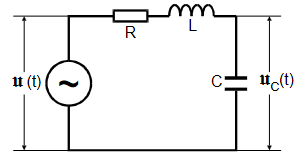
\includegraphics[width = 0.5\textwidth]{pics/Erzwungen.png}
\end{figure}
Es kommt zu einer Inhomogenität in der 
Differentialgleichung. Bei der Berechnung der Spannung an dem Kondensator, folgt die Frequenzabhängigkeit
\begin{equation}
    U_\text{C}(\omega)= \frac{U_0}{\sqrt{\left(1-LC\omega^2\right)}^2 + \omega^2 R^2 C^2} \, .
\end{equation}
Die Spannung hat ein Maximum bei $\omega=\omega_\text{res}$ mit 
\begin{equation}
    \omega_\text{res}= \frac{1}{2 \pi} \sqrt{\frac{1}{L C} - \frac{R^2}{4 L^2}} \, ,
\end{equation}
dass Resonanzüberhöhung genannt wird. Mit Hilfe der beiden Frequenzen $\omega_+$ und $\omega_-$, an denen $U_\text{C}$ auf den Bruchteil $\sfrac{1}{\sqrt{2}}$
abgefallen ist, lässt sich die Güte 
\begin{equation}
    q=\frac{\omega_\text{res}}{\omega_+ - \omega_-}
\end{equation}
berechnen. Dabei können $\omega_+$ und $\omega_-$ berechnet werden mit
\begin{equation}
    \omega_\pm= \pm \frac{R}{4 \pi L} + \frac{1}{2\pi} \sqrt{\frac{1}{L C} + \frac{R^2}{4 L^2}} \, .
\end{equation}
Angenähert ergibt sich $\omega_+ - \omega_- \approx \frac{R}{L}$ für die Differenz.